\documentclass[twocolumn,a4j]{jarticle}
\usepackage[dvipdfmx]{graphicx}

\title{DAOの機能改善提案(abstract)}
\author{九州工業大学 情報工学部 荒木研究室 津田 匠貴}
\date{2021年11月29日}
\begin{document}
\maketitle
\section{はじめに}
DAO(Decentralized Autonomous Organization:自立分散型組織)は経済的な共通目的を持った匿名の個人らが中央集権的な管理主体を持たず、特定の国や法定通貨に依存せずに活動を行う組織である。
このような組織形態を可能にしているのがブロックチェーン技術によって可能になった独自トークンの発行や分散台帳としての記録機能である。

自立分散的に機能するまでは株式会社やNPOなどの中央集権的組織が主体となって運営する。
彼らによる不正を防止し、その活動を早期にコミュニティへ移管することが求められるため、本研究では現在の一般的なDAOをいかにして理想形に改善できるのか考える。
具体的には、メンバーシップの導入とゼロ知識証明をを用いた投票、内部告発機能を提案する。
\section{メンバーシップの導入}
DAOのメンバーとその他の線引きをするために以下のメンバーシップを導入する。
\begin{figure}[htbp]
  \begin{center}
    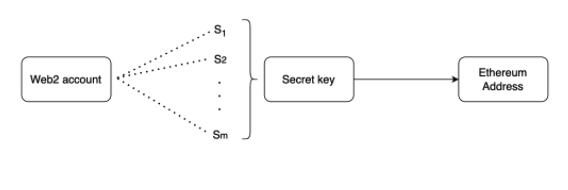
\includegraphics[width=80mm]{account.png}
    \caption{アカウント管理モデル}
  \end{center}
\end{figure}

内部告発において、コミュニティ全体で判決を決定し被告へ制裁を行うために以下のような設計となっている。
\begin{itemize}
  \item 1つのSecret keyをm個のsecret shareに分割
  \item 1つのWeb2 account(TwitterやTelegramのアカウント)につき、m個のsecret shareを紐付ける
  \item それぞれのWeb2 accountとsecret shareのペアはm人のメンバーに配られる
  \item n個のsecret shareが集まればシャミアの秘密分散法により、被告発者の秘密鍵が再現できる
  \item (n,m)の値は自由に変更できる(n≦m≦総メンバー数)
  \item Ethereum AddressからWeb2 accountを特定することはできない
\end{itemize}
\section{DAOにおける投票}
プログラムの改善提案や助成金の決定など、DAOの方向性を自分たちで決める民主的な手段として投票はDAOに欠かせない機能であり、多くのDAOではこの機能を提供している。
\begin{figure}[htbp]
  \begin{center}
    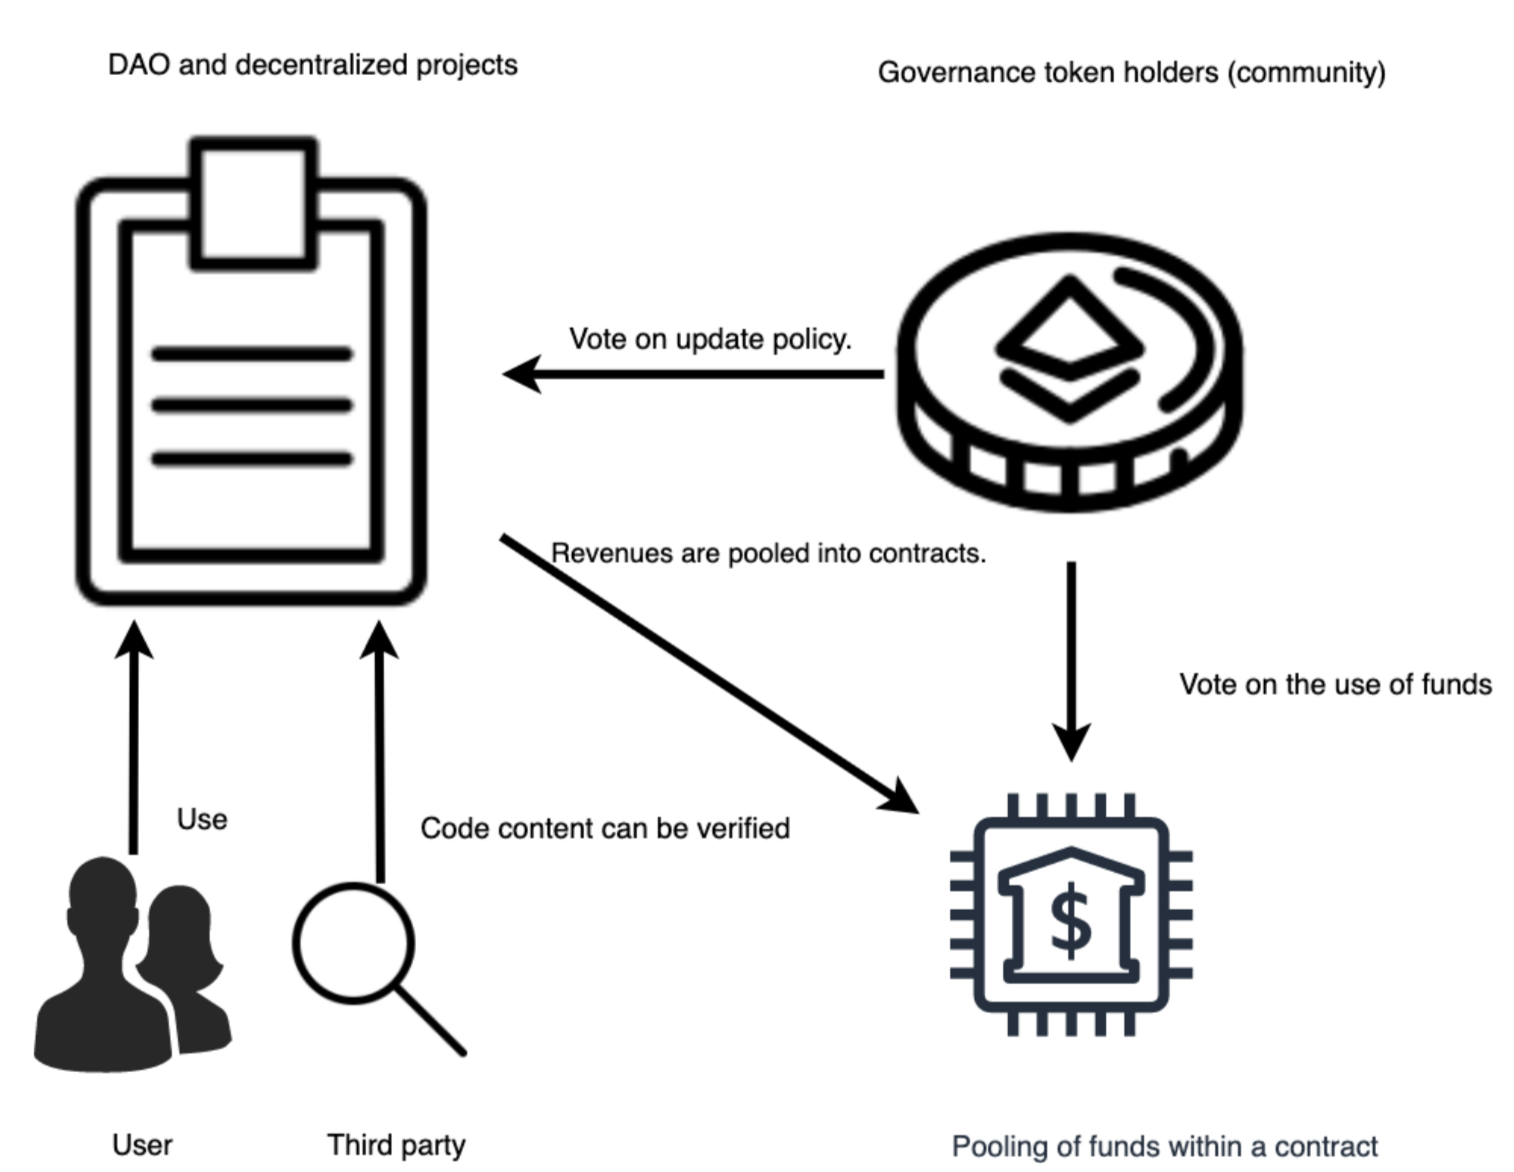
\includegraphics[width=80mm]{vote.png}
    \caption{DAOにおける投票の仕組み}
  \end{center}
\end{figure}
投票にはガバナンストークンを使う例がほとんどあり、その取引履歴は分散台帳に記録されているため誰でも確認できる。
そのため、個人の資産の流れや投票傾向を他者が把握でき、プライバシーの懸念がある。これを解決する手段としては投票にガバナンストークンを使用せず、純粋な投票機能のみを提供することが挙げられる。
「ガバナンストークンを持っていること」=「DAOのメンバーであること」というようにクレデンシャルとして扱われているため、「投票機能」「メンバーシップの識別」に機能を分ける。

\section{DAOにおける内部告発}
DAOの内部告発におけるフローチャートは以下のようになる。
\begin{figure}[htbp]
  \begin{center}
    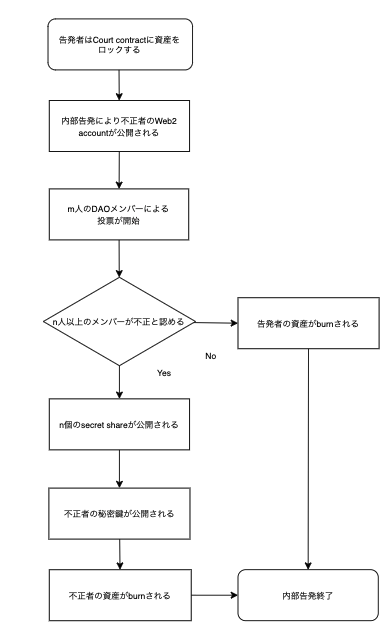
\includegraphics[width=80mm]{flow.png}
    \caption{内部告発の流れ}
  \end{center}
\end{figure}
\begin{enumerate}
  \item 告発者を報復から守るために、匿名性を担保する
  \item 告発内容に対する判決は、メンバーの投票によって決定される
  \item Web3で起きるインシデントは事後の解決や制裁が難しいうえ、Web3上の情報のみで事前に察知することは困難である。
  \item そのため、Web2でのチャット内容などから起きうるインシデントをWeb3上のコミュニティの判断で予見し、裁きたい
\end{enumerate}



\section{用語解説}
\begin{itemize}
  \item トークン:ブロックチェーンによって発行、管理される資産や権利のことを指す。
  \item ガバナンストークン:DAOが発行するトークンのことを指す。これは、純粋な資産としての利用のほかに方向性を決める投票権としても利用される。ï
  \item スマートコントラクト:ブロックチェーン上で実行されるプログラムであり、トークンの移動や売買の契約を自動で執行できる。
  \item Web3:ブロックチェーンの登場により唱えられた分散型のwebサービスを総称した概念であり、中央集権的なプラットーフォームに依存しているサービスはWeb2と呼ぶ。
  \item シャミアの秘密分散法:秘密の値をm個のsecret shareに分散しユーザに配布する。閾値以上のsecret shareが再び集まれば秘密の値を復元できる。
  \item ゼロ知識証明:ある命題の答えを知っていることを、その答え自体を示さずに証明する方法
\end{itemize}


\begin{thebibliography}{99}
  \bibitem{sincho} 太宰治、『走れメロス』、新潮(1940年5月号)
  \bibitem{chikuma} 太宰治、太宰治全集3(ちくま文庫)、筑摩書房(1988).
  \bibitem{schiller} Friedrich von Schiller, バラード¥textit{de:Die B¥"{u}rgschaft}, 1815.
\end{thebibliography}

\end{document}
